\documentclass[]{book}
\usepackage{lmodern}
\usepackage{amssymb,amsmath}
\usepackage{ifxetex,ifluatex}
\usepackage{fixltx2e} % provides \textsubscript
\ifnum 0\ifxetex 1\fi\ifluatex 1\fi=0 % if pdftex
  \usepackage[T1]{fontenc}
  \usepackage[utf8]{inputenc}
\else % if luatex or xelatex
  \ifxetex
    \usepackage{mathspec}
  \else
    \usepackage{fontspec}
  \fi
  \defaultfontfeatures{Ligatures=TeX,Scale=MatchLowercase}
\fi
% use upquote if available, for straight quotes in verbatim environments
\IfFileExists{upquote.sty}{\usepackage{upquote}}{}
% use microtype if available
\IfFileExists{microtype.sty}{%
\usepackage{microtype}
\UseMicrotypeSet[protrusion]{basicmath} % disable protrusion for tt fonts
}{}
\usepackage[margin=1in]{geometry}
\usepackage{hyperref}
\hypersetup{unicode=true,
            pdftitle={YaRrr! The Pirate's Guide to R},
            pdfauthor={Nathaniel D. Phillips},
            pdfborder={0 0 0},
            breaklinks=true}
\urlstyle{same}  % don't use monospace font for urls
\usepackage{natbib}
\bibliographystyle{apalike}
\usepackage{color}
\usepackage{fancyvrb}
\newcommand{\VerbBar}{|}
\newcommand{\VERB}{\Verb[commandchars=\\\{\}]}
\DefineVerbatimEnvironment{Highlighting}{Verbatim}{commandchars=\\\{\}}
% Add ',fontsize=\small' for more characters per line
\usepackage{framed}
\definecolor{shadecolor}{RGB}{248,248,248}
\newenvironment{Shaded}{\begin{snugshade}}{\end{snugshade}}
\newcommand{\KeywordTok}[1]{\textcolor[rgb]{0.13,0.29,0.53}{\textbf{{#1}}}}
\newcommand{\DataTypeTok}[1]{\textcolor[rgb]{0.13,0.29,0.53}{{#1}}}
\newcommand{\DecValTok}[1]{\textcolor[rgb]{0.00,0.00,0.81}{{#1}}}
\newcommand{\BaseNTok}[1]{\textcolor[rgb]{0.00,0.00,0.81}{{#1}}}
\newcommand{\FloatTok}[1]{\textcolor[rgb]{0.00,0.00,0.81}{{#1}}}
\newcommand{\ConstantTok}[1]{\textcolor[rgb]{0.00,0.00,0.00}{{#1}}}
\newcommand{\CharTok}[1]{\textcolor[rgb]{0.31,0.60,0.02}{{#1}}}
\newcommand{\SpecialCharTok}[1]{\textcolor[rgb]{0.00,0.00,0.00}{{#1}}}
\newcommand{\StringTok}[1]{\textcolor[rgb]{0.31,0.60,0.02}{{#1}}}
\newcommand{\VerbatimStringTok}[1]{\textcolor[rgb]{0.31,0.60,0.02}{{#1}}}
\newcommand{\SpecialStringTok}[1]{\textcolor[rgb]{0.31,0.60,0.02}{{#1}}}
\newcommand{\ImportTok}[1]{{#1}}
\newcommand{\CommentTok}[1]{\textcolor[rgb]{0.56,0.35,0.01}{\textit{{#1}}}}
\newcommand{\DocumentationTok}[1]{\textcolor[rgb]{0.56,0.35,0.01}{\textbf{\textit{{#1}}}}}
\newcommand{\AnnotationTok}[1]{\textcolor[rgb]{0.56,0.35,0.01}{\textbf{\textit{{#1}}}}}
\newcommand{\CommentVarTok}[1]{\textcolor[rgb]{0.56,0.35,0.01}{\textbf{\textit{{#1}}}}}
\newcommand{\OtherTok}[1]{\textcolor[rgb]{0.56,0.35,0.01}{{#1}}}
\newcommand{\FunctionTok}[1]{\textcolor[rgb]{0.00,0.00,0.00}{{#1}}}
\newcommand{\VariableTok}[1]{\textcolor[rgb]{0.00,0.00,0.00}{{#1}}}
\newcommand{\ControlFlowTok}[1]{\textcolor[rgb]{0.13,0.29,0.53}{\textbf{{#1}}}}
\newcommand{\OperatorTok}[1]{\textcolor[rgb]{0.81,0.36,0.00}{\textbf{{#1}}}}
\newcommand{\BuiltInTok}[1]{{#1}}
\newcommand{\ExtensionTok}[1]{{#1}}
\newcommand{\PreprocessorTok}[1]{\textcolor[rgb]{0.56,0.35,0.01}{\textit{{#1}}}}
\newcommand{\AttributeTok}[1]{\textcolor[rgb]{0.77,0.63,0.00}{{#1}}}
\newcommand{\RegionMarkerTok}[1]{{#1}}
\newcommand{\InformationTok}[1]{\textcolor[rgb]{0.56,0.35,0.01}{\textbf{\textit{{#1}}}}}
\newcommand{\WarningTok}[1]{\textcolor[rgb]{0.56,0.35,0.01}{\textbf{\textit{{#1}}}}}
\newcommand{\AlertTok}[1]{\textcolor[rgb]{0.94,0.16,0.16}{{#1}}}
\newcommand{\ErrorTok}[1]{\textcolor[rgb]{0.64,0.00,0.00}{\textbf{{#1}}}}
\newcommand{\NormalTok}[1]{{#1}}
\usepackage{longtable,booktabs}
\usepackage{graphicx,grffile}
\makeatletter
\def\maxwidth{\ifdim\Gin@nat@width>\linewidth\linewidth\else\Gin@nat@width\fi}
\def\maxheight{\ifdim\Gin@nat@height>\textheight\textheight\else\Gin@nat@height\fi}
\makeatother
% Scale images if necessary, so that they will not overflow the page
% margins by default, and it is still possible to overwrite the defaults
% using explicit options in \includegraphics[width, height, ...]{}
\setkeys{Gin}{width=\maxwidth,height=\maxheight,keepaspectratio}
\IfFileExists{parskip.sty}{%
\usepackage{parskip}
}{% else
\setlength{\parindent}{0pt}
\setlength{\parskip}{6pt plus 2pt minus 1pt}
}
\setlength{\emergencystretch}{3em}  % prevent overfull lines
\providecommand{\tightlist}{%
  \setlength{\itemsep}{0pt}\setlength{\parskip}{0pt}}
\setcounter{secnumdepth}{5}
% Redefines (sub)paragraphs to behave more like sections
\ifx\paragraph\undefined\else
\let\oldparagraph\paragraph
\renewcommand{\paragraph}[1]{\oldparagraph{#1}\mbox{}}
\fi
\ifx\subparagraph\undefined\else
\let\oldsubparagraph\subparagraph
\renewcommand{\subparagraph}[1]{\oldsubparagraph{#1}\mbox{}}
\fi

%%% Use protect on footnotes to avoid problems with footnotes in titles
\let\rmarkdownfootnote\footnote%
\def\footnote{\protect\rmarkdownfootnote}

%%% Change title format to be more compact
\usepackage{titling}

% Create subtitle command for use in maketitle
\newcommand{\subtitle}[1]{
  \posttitle{
    \begin{center}\large#1\end{center}
    }
}

\setlength{\droptitle}{-2em}
  \title{YaRrr! The Pirate's Guide to R}
  \pretitle{\vspace{\droptitle}\centering\huge}
  \posttitle{\par}
  \author{Nathaniel D. Phillips}
  \preauthor{\centering\large\emph}
  \postauthor{\par}
  \predate{\centering\large\emph}
  \postdate{\par}
  \date{2017-02-22}

\usepackage{booktabs}
\usepackage{amsthm}
\makeatletter
\def\thm@space@setup{%
  \thm@preskip=8pt plus 2pt minus 4pt
  \thm@postskip=\thm@preskip
}
\makeatother

\begin{document}
\maketitle

{
\setcounter{tocdepth}{1}
\tableofcontents
}
\chapter{Preface}\label{intro}

\begin{center}
\includegraphics[width=0.75\linewidth]{images/YaRrr_Cover} \end{center}

The purpose of this book is to help you learn R from the ground-up.

\section{Where did this book come
from?}\label{where-did-this-book-come-from}

Let me make something very, very clear\ldots{}

\emph{I did not write this book}.

This whole story started in the Summer of 2015. I was taking a late
night swim on the Bodensee in Konstanz and saw a rusty object sticking
out of the water. Upon digging it out, I realized it was an ancient
usb-stick with the word YaRrr inscribed on the side. Intrigued, I
brought it home and plugged it into my laptop. Inside the stick, I found
a single pdf file written entirely in pirate-speak. After watching
several pirate movies, I learned enough pirate-speak to begin
translating the text to English. Sure enough, the book turned out to be
an introduction to R called The Pirate's Guide to R.

This book clearly has both massive historical and pedagogical
significance. Most importantly, it turns out that pirates were
programming in R well before the earliest known advent of computers. Of
slightly less significance is that the book has turned out to be a
surprisingly up-to-date and approachable introductory text to R. For
both of these reasons, I felt it was my duty to share the book with the
world.

If you or spot any typos or errors, or have any recommendations for
future versions of the book, please write me at YaRrr.Book@gmail.com or
tweet me @YaRrrBook.

\section{Who is this book for?}\label{who-is-this-book-for}

While this book was originally written for pirates, I think that anyone
who wants to learn R can benefit from this book. If you haven't had an
introductory course in statistics, some of the later statistical
concepts may be difficult, but I'll try my best to add brief
descriptions of new topics when necessary. Likewise, if R is your first
programming language, you'll likely find the first few chapters quite
challenging as you learn the basics of programming. However, if R is
your first programming language, that's totally fine as what you learn
here will help you in learning other languages as well (if you choose
to). Finally, while the techniques in this book apply to most data
analysis problems, because my background is in experimental psychology I
will cater the course to solving analysis problems commonly faced in
psychological research.

\textbf{What this book is}

This book is meant to introduce you to the basic analytical tools in R,
from basic coding and analyses, to data wrangling, plotting, and
statistical inference.

\textbf{What this book is not}

This book does not cover any one topic in extensive detail. If you are
interested in conducting analyses or creating plots not covered in the
book, I'm sure you'll find the answer with a quick Google search!

\section{Why is R so great?}\label{why-is-r-so-great}

As you've already gotten this book, you probably already have some idea
why R is so great. However, in order to help prevent you from giving up
the first time you run into a programming wall, let me give you a few
more reasons:

\begin{enumerate}
\def\labelenumi{\arabic{enumi}.}
\item
  R is 100\% free and as a result, has a huge support community. Unlike
  SPSS, Matlab, Excel and JMP, R is, and always will be completely free.
  This doesn't just help your wallet - it means that a huge community of
  R programmers will constantly develop an distribute new R
  functionality and packages at a speed that leaves all those other
  packages in the dust! Unlike Fight Club, the first rule of R is ``Do
  talk about R!'' The size of the R programming community is staggering.
  If you ever have a question about how to implement something in R, a
  quick
  Poogle\footnote{I am in the process of creating Poogle - Google for Pirates. Kickstarter page coming soon...}
  search will lead you to your answer virtually every single time.
\item
  R is the presnt, and future of statistical programming. To illustrate
  this, look at the following three figures. These are Google trend
  searches for three terms: R Programming, Matlab, and SPSS. Try and
  guess which one is which.
\end{enumerate}

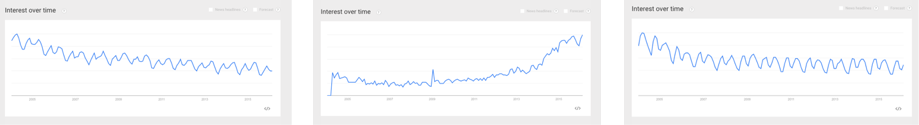
\includegraphics{images/googletrends.png}

\begin{enumerate}
\def\labelenumi{\arabic{enumi}.}
\setcounter{enumi}{2}
\item
  R is incredibly versatile. You can use R to do everything from
  calculating simple summary statistics, to performing complex
  simulations to creating gorgeous plots like the chord diagram on the
  right. If you can imagine an analytical task, you can almost certainly
  implement it in R.
\item
  Using RStudio, a program to help you write R code, You can easily and
  seamlessly combine R code, analyses, plots, and written text into
  elegant documents all in one place using Sweave (R and Latex) or
  RMarkdown. In fact, I translated this entire book (the text,
  formatting, plots, code\ldots{}yes, everything) in RStudio using
  Sweave. With RStudio and Sweave, instead of trying to manage two or
  three programs, say Excel, Word and (sigh) SPSS, where you find
  yourself spending half your time copying, pasting and formatting data,
  images and test, you can do everything in one place so nothing gets
  misread, mistyped, or forgotten.
\end{enumerate}

\begin{Shaded}
\begin{Highlighting}[]
\NormalTok{circlize::}\KeywordTok{chordDiagram}\NormalTok{(}\KeywordTok{matrix}\NormalTok{(}\KeywordTok{sample}\NormalTok{(}\DecValTok{10}\NormalTok{), }
                              \DataTypeTok{nrow =} \DecValTok{2}\NormalTok{, }\DataTypeTok{ncol =} \DecValTok{5}\NormalTok{))}
\end{Highlighting}
\end{Shaded}

\begin{figure}[htbp]
\centering
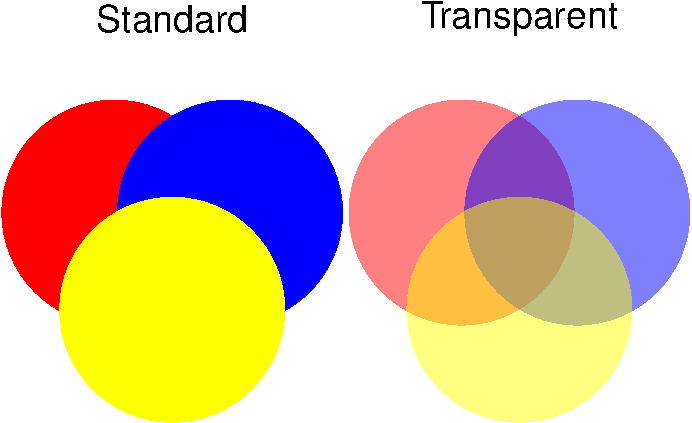
\includegraphics{YaRrr_files/figure-latex/unnamed-chunk-3-1.pdf}
\caption{\label{fig:unnamed-chunk-3}A super cool chord diagram from the
circlize package}
\end{figure}

\begin{enumerate}
\def\labelenumi{\arabic{enumi}.}
\setcounter{enumi}{4}
\item
  Analyses conducted in R are transparent, easily shareable, and
  reproducible. If you ask an SPSS user how they conducted a specific
  analyses, they will either A) Not remember, B) Try (nervously) to
  construct an analysis procedure on the spot that makes sense - which
  may or may not correspond to what they actually did months or years
  ago, or C) Ask you what you are doing in their house. I used to
  primarily use SPSS, so I speak from experience on this. If you ask an
  R user (who uses good programming techniques!) how they conducted an
  analysis, they should always be able to show you the exact code they
  used. Of course, this doesn't mean that they used the appropriate
  analysis or interpreted it correctly, but with all the original code,
  any problems should be completely transparent!
\item
  And most importantly of all, R is the programming language of choice
  for pirates.
\end{enumerate}

\section{R is like a
relationship\ldots{}}\label{r-is-like-a-relationship}

Yes, R is very much like a relationship. Like relationships, there are
two major truths to R programming:

\begin{figure}

{\centering 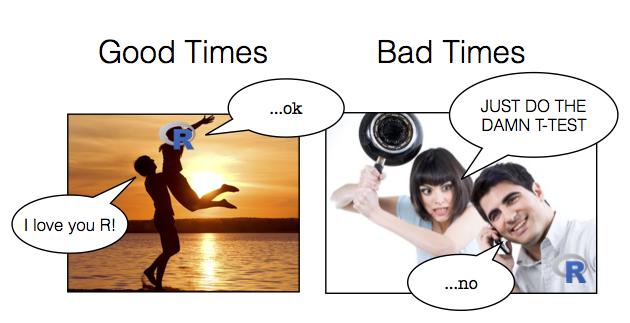
\includegraphics{images/rrelationship} 

}

\caption{Yep, R will become both your best friend and your worst nightmare. The bad times will make the good times oh so much sweeter.}\label{fig:unnamed-chunk-4}
\end{figure}

\begin{enumerate}
\def\labelenumi{\arabic{enumi}.}
\item
  There is nothing more \emph{frustrating} than when your code does
  \emph{not} work
\item
  There is nothing more \emph{satisfying} than when your code
  \emph{does} work!
\end{enumerate}

Anything worth doing, from losing weight to getting a degree, takes
time. Learning R is no different. Especially if this is your first
experience programming, you are going to experience a \emph{lot} of
headaches when you get started. You will run into error after error and
pound your fists against the table screaming: ``WHY ISN'T MY CODE
WORKING?!?!? There must be something wrong with this stupid
software!!!'' You will spend hours trying to find a bug in your code,
only to find that - frustratingly enough, you had had an extra space or
missed a comma somewhere. You'll then wonder why you ever decided to
learn R when (::sigh::) SPSS was so ``nice and easy.''

\begin{figure}

{\centering 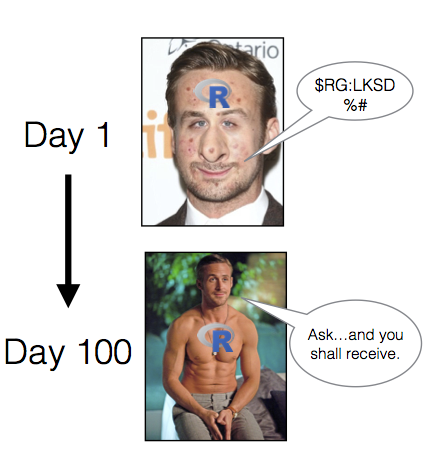
\includegraphics{images/gosling} 

}

\caption{When you first meet R, it will look so fugly that you'll wonder if this is all some kind of sick joke. But trust me, once you learn how to talk to it, and clean it up a bit, all your friends will be crazy jealous.}\label{fig:unnamed-chunk-5}
\end{figure}

\textbf{Fun Fact!} SPSS stands for ``Shitty Piece of Shitty Shit''. True
story.

This is perfectly normal! Don't get discouraged and DON'T GO BACK TO
SPSS! That would be quitting on exercise altogether because you had a
tough workout.

Trust me, as you gain more programming experience, you'll experience
fewer and fewer bugs (though they'll never go away completely). Once you
get over the initial barriers, you'll find yourself conducting analyses
much, much faster than you ever did before.

\section{Who am I?}\label{who-am-i}

\begin{figure}

{\centering 
\includegraphics[width=7.49in]{images/beer} 

}

\caption{Like a pirate, I work best with a mug of beer within arms' reach.}\label{fig:unnamed-chunk-6}
\end{figure}

My name is Nathaniel -- not Nathan\ldots{}not Nate\ldots{}and
\emph{definitely} not Nat. I am a psychologist with a background in
statistics and judgment and decision making. You can find my R (and
non-R) related musings at \url{http://ndphillips.github.io}

\chapter{Getting Started}\label{started}

\chapter{Jump In!}\label{jumpin}

\chapter{The Basics}\label{basics}

\chapter{Scalers and vectors}\label{scalersvectors}

\chapter{Vector functions}\label{vectorfunctions}

\chapter{Indexing Vectors with {[} {]}}\label{vectorindexing}

\chapter{Matrices and Dataframes}\label{matricesdataframes}

\chapter{Test your R might!
Solutions}\label{test-your-r-might-solutions}

\chapter{Placeholder}\label{placeholder}

\bibliography{packages.bib,book.bib}


\end{document}
